\chapter{Конструкторский раздел}
\label{cha:design}

%В данном разделе спроектирована база данных и соответствующее приложение на основе выделенных сущностей и их свойств из предыдущего раздела.

\section{Ролевая модель}

Ролевая модель используется для реализации системы безопасности сервера базы данных и  позволяет разрешать или запрещать тем или иным группам пользователей работу с объектами базы данных. %Таким образом, каждой группе пользователей (роли) ставится в соответвие набор привелегий. 

%Процесс предоставления доступа осуществляется путем реализации системы аутентификации и авторизации в системе.

В рамках поставленной задачи выделены следующие роли:

\begin{enumerate}
	\item Пациент - роль, которой соответствует функционал записи на прием к врачу, просмотра медицинской карты, личного кабинета и активных заявок на прием.
	\item Доктор - роль, которой соответствует функционал обработки заявок на прием, назначения диагнозов и лекарств, а также просмотр личного кабинета.
	\item Администратор - роль, которой соответствует функционал регистрации новых пользователей в системе с ролями <<Доктор>> и <<Администратор>>, функционал просмотра зарегистрированных пользователей в системе с любой ролью, а также просмотр статистики о заболеваемости.
\end{enumerate}

%\clearpage

\subsection*{Варианты использования системы}

На рисунках 2.1-2.4 представлены диаграммы вариантов использования системы в соответствии с выделенными типами пользователей.

\begin{figure}[!h]
	\center{
\includegraphics[scale=0.95]{assets/use_case_unauth.pdf}}
	\caption{Диаграмма вариантов использования системы для незарегистрированного пользователя}
\end{figure}

%На рисунке 2.1 представлена диаграмма вариантов использования системы для пользователя с ролью <<Доктор>>.
\clearpage

\begin{figure}[!t]
	\center{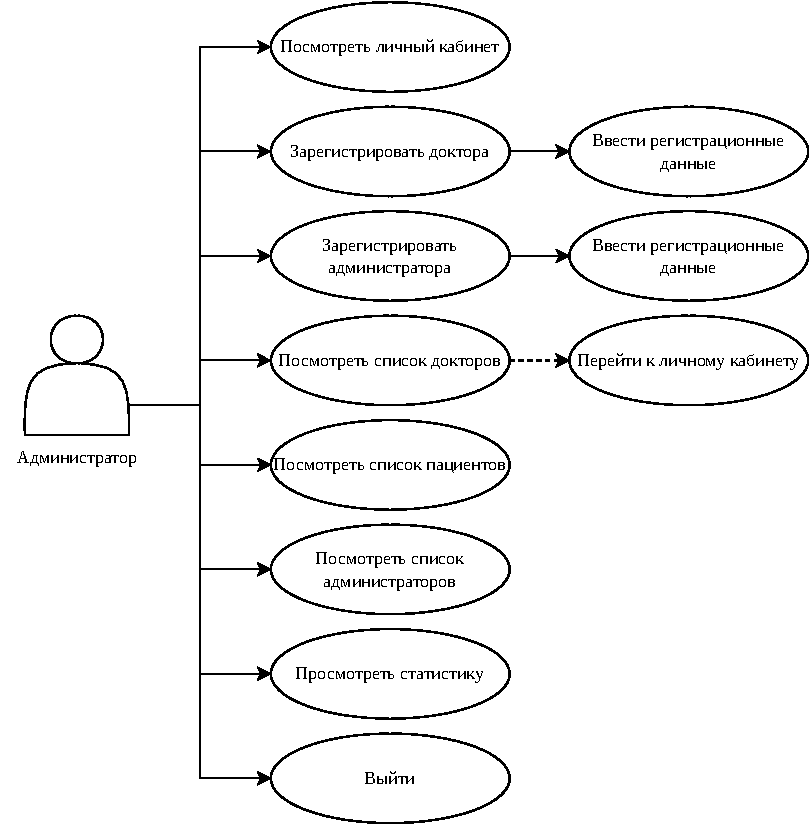
\includegraphics[scale=1]{assets/use_case_admin.pdf}}
	\caption{Диаграмма вариантов использования системы для администратора}
\end{figure}

\begin{figure}[!t]
	\center{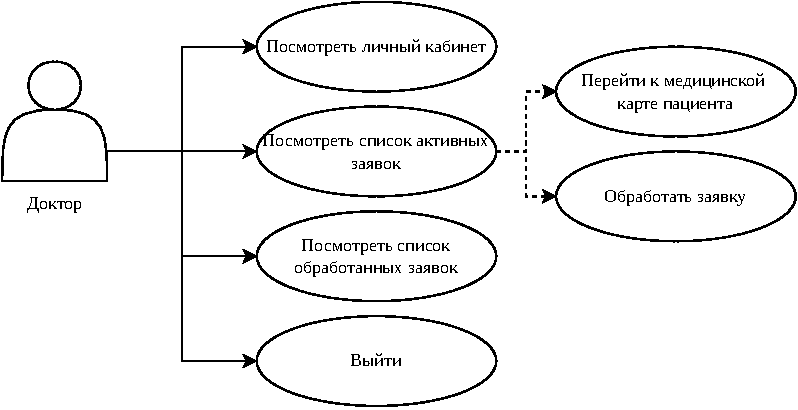
\includegraphics[scale=1]{assets/use_case_doctor.pdf}}
	\caption{Диаграмма вариантов использования системы для доктора}
\end{figure}

%На рисунке 2.1 представлена диаграмма вариантов использования системы для пользователя с ролью <<Пациент>>.

\begin{figure}[!t]
	\center{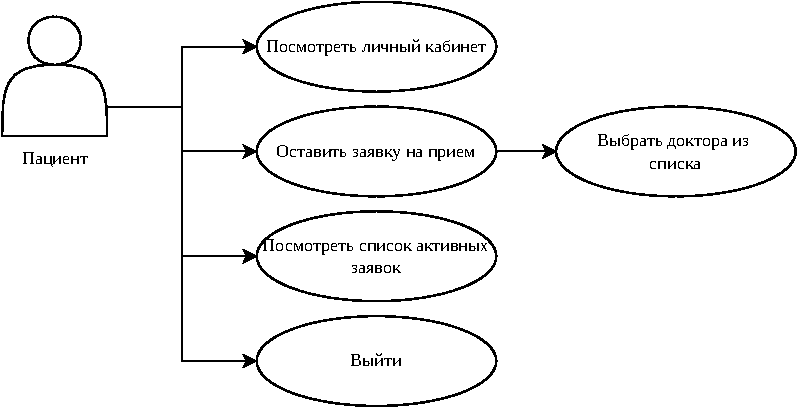
\includegraphics[scale=1]{assets/use_case_patient.pdf}}
	\caption{Диаграмма вариантов использования системы для пациента}
\end{figure}

%На рисунке 2.1 представлена диаграмма вариантов использования системы для пользователя с ролью <<Администратор>>.

%\begin{figure}[!h]
%	\center{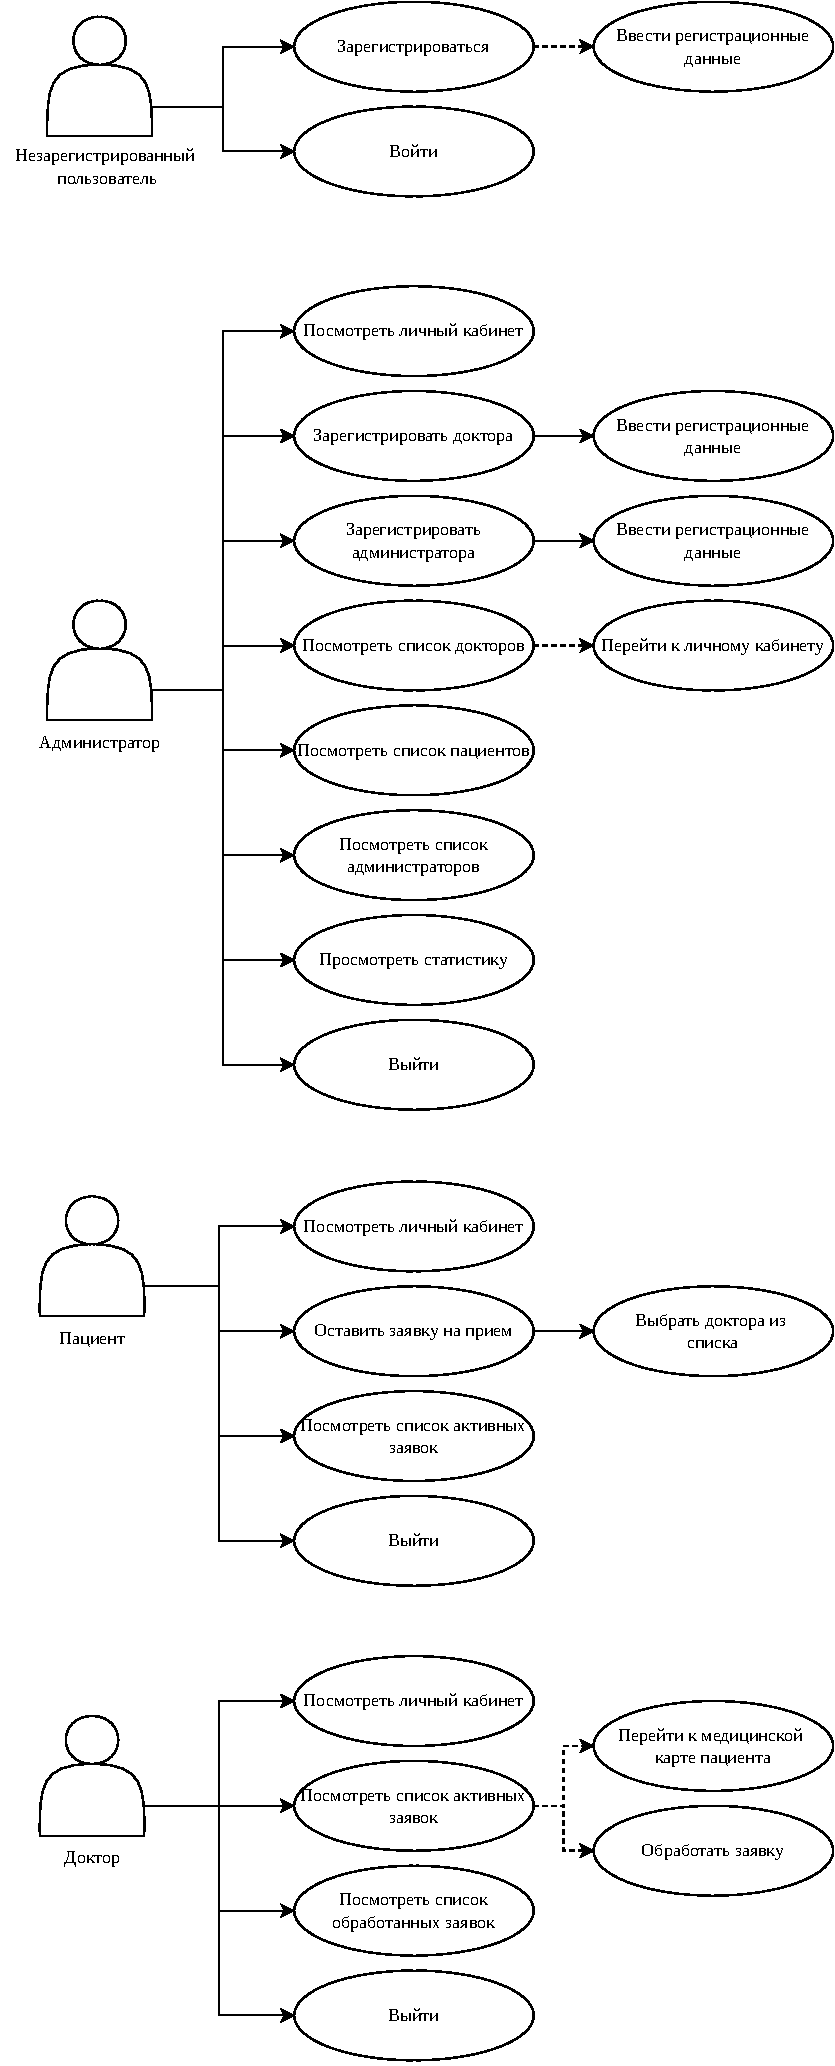
\includegraphics[scale=0.6]{assets/use_case.pdf}}
%	\caption{Диаграмма вариантов использования системы различными типами пользователей}
%\end{figure}
%
%Во время запуска приложения предоставляется функционал для незарегистрированного пользователя: возможность зарегистрироваться в системе или войти в нее.
%
%Пациент может зарегистрироваться с помощью заполнения стартовой анкеты на главной странице сайта. После успешной регистрации пациенту предоставляется меню, позволяющее просмотреть данные о себе в личном кабинете, оставить заявку на прием или посмотреть свои активные заявки. Также можно выйти из системы.
%
%Администратор может зарегистрироваться в системе, введя специальный адрес в системе, либо же его может зарегистрировать в системе другой администратор. Также администратор может зарегстрировать доктора в системе. 
%
%Администратор имеет возможность просмотреть информацию обо всех зарегистрированных пользователях в системе и обо всех обработанных заявках на прием. Только администратор может посмотреть статистику о заболеваемости.
%
%После входа в систему доктор может управлять своими заявками: смотреть активные заявки, обрабатывать их, смотреть карты пациентов.

\section{Проектирование базы данных}

На рисунке 2.5 представлена ER-диаграмма разрабатываемой базы данных, спроектированная на основе выделенных сущностей и их свойств из предыдущего раздела.

\begin{figure}[!h]
	\center{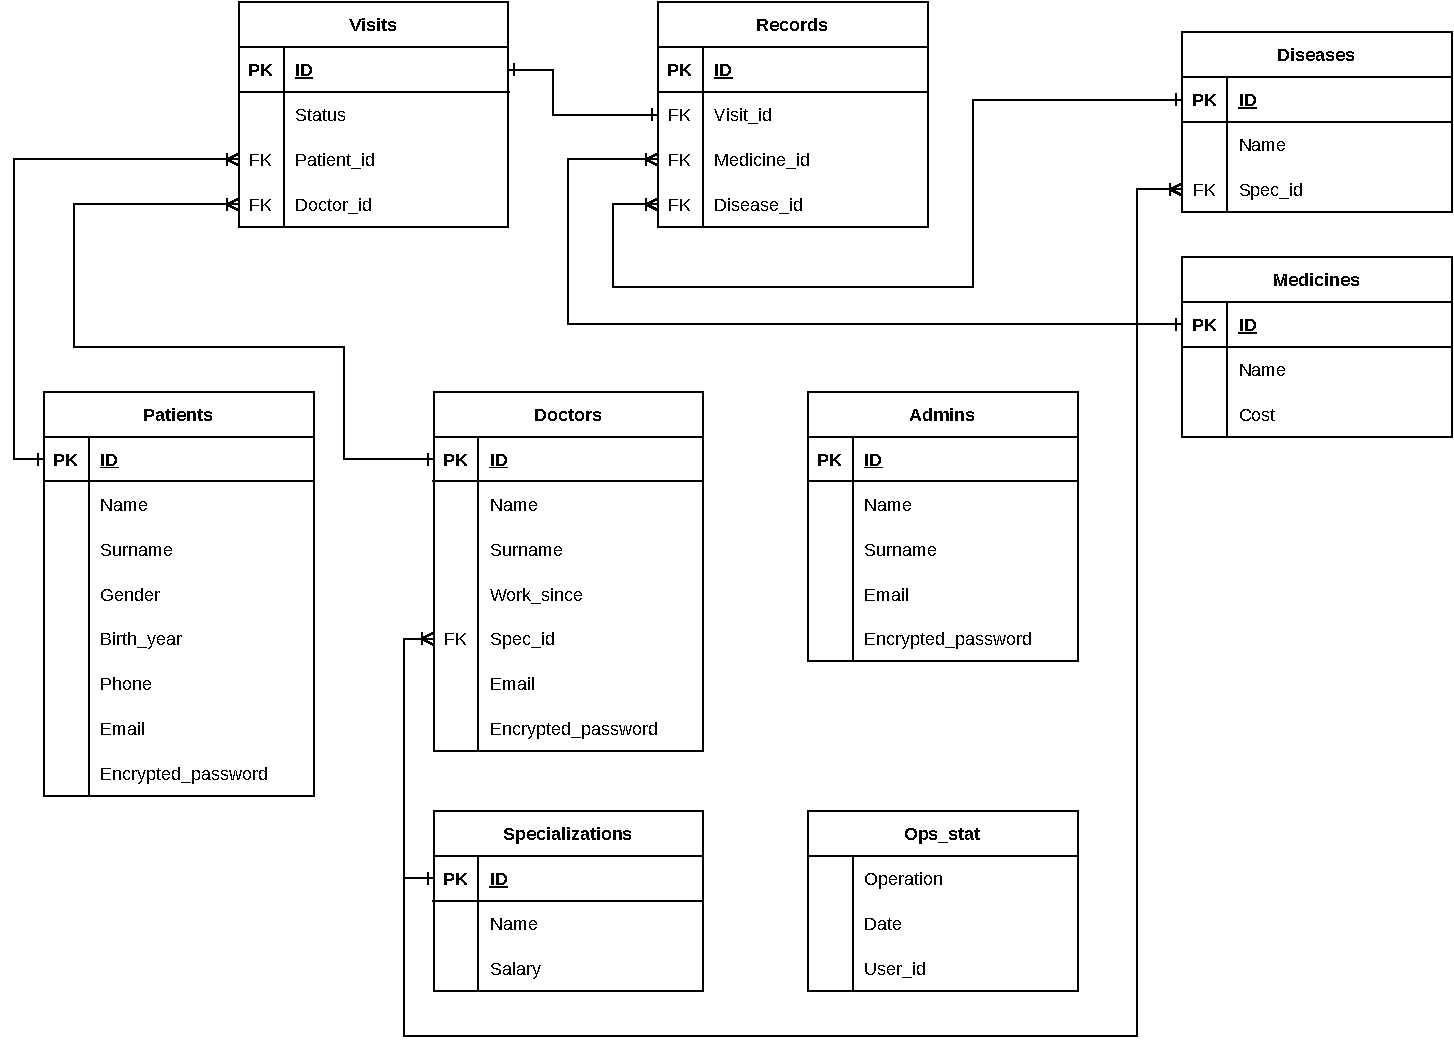
\includegraphics[scale=0.65]{assets/erd.pdf}}
	\caption{ERD-диаграмма разрабатываемой базы данных}
\end{figure}

Далее приведено описание полей каждой таблицы из базы данных. Соответствующий скрипт можно посмотреть в приложении А.

\subsection*{Таблица Medicines}

Данная таблица используется для описания назначаемого пациенту медицинского препарата.

Значения полей:

\begin{itemize}
	\item ID - уникальный идентификатор медицинского препарата, целочисленный тип.
	\item Name - наименование, строковый тип.
	\item Cost - цена (в российских рублях), целочисленный тип.
\end{itemize}

\subsection*{Таблица Specializations}

Данная таблица используется для описания врачебной специализации.

Значения полей:

\begin{itemize}
	\item ID - уникальный идентификатор специализации, целочисленный тип.
	\item Name - наименование, строковый тип.
	\item Salary - зарплата доктора с соответствующей специализацией (в российских рублях), целочисленный тип.
\end{itemize}

\subsection*{Таблица Diseases}

Данная таблица используется для описания диагностируемого заболевания.

Значения полей:

\begin{itemize}
	\item ID - уникальный идентификатор заболевания, целочисленный тип.
	\item Name - наименование, строковый тип.
	\item Spec\_id - идентификатор специализации, к кототорой относится заболевание. Является внешним ключом относительно поля ID таблицы Specializations, целочисленный тип.
\end{itemize}

\subsection*{Таблица Admins}

Данная таблица используется для описания типа пользователя <<Администратор>>.

Значения полей:

\begin{itemize}
	\item ID - уникальный идентификатор пользователя <<Администратор>>, целочисленный тип.
	\item Name - имя, строковый тип.
	\item Surname - фамилия, строковый тип.
	\item Email - адрес электорнной почты, строковый тип.
	\item Encrypted\_password - зашифрованный пароль, строковый тип.
\end{itemize}

\subsection*{Таблица Doctors}

Данная таблица используется для описания типа пользователя <<Доктор>>.

Значения полей:

\begin{itemize}
	\item ID - уникальный идентификатор пользователя <<Доктор>>, целочисленный тип.
	\item Name - имя, строковый тип.
	\item Surname - фамилия, строковый тип.
	\item Work\_since - год начала врачебной практики, целочисленный тип.
	\item Spec\_id - идентификатор специализации доктора. Является внешним ключом относительно поля ID таблицы Spacializations, целочисленный тип.
	\item Email - адрес электорнной почты, строковый тип.
	\item Encrypted\_password - зашифрованный пароль, строковый тип.
\end{itemize}

\subsection*{Таблица Patients}

Данная таблица используется для описания типа пользователя <<Пациент>>.

Значения полей:

\begin{itemize}
	\item ID - уникальный идентификатор пользователя <<Доктор>>, целочисленный тип.
	\item Name - имя, строковый тип.
	\item Surname - фамилия, строковый тип.
	\item Gender - пол, строковый тип.
	\item Birth\_year - год рождения, целочисленный тип.
	\item Phone - номер телефона, строковый тип.
	\item Email - адрес электорнной почты, строковый тип.
	\item Encrypted\_password - зашифрованный пароль, строковый тип.
\end{itemize}

\subsection*{Таблица Visits}

Данная таблица используется для описания приема пациента.

Значения полей:

\begin{itemize}
	\item ID - уникальный идентификатор приема, целочисленный тип.
	\item Status - статус приема. Может принимать одно из двух возможных значений: <<Активный>> (запланированный, еще не совершившийся) и <<Обработанный>> (совершившийся прием), строковый тип.
	\item Patient\_id - идентификатор пациента. Является внешним ключом относительно поля ID таблицы Patients, целочисленный тип.
	\item Doctor\_id - идентификатор доктора. Является внешним ключом относительно поля ID таблицы Doctors, целочисленный тип.
\end{itemize}

\subsection*{Таблица Records}

Данная таблица используется для описания записи из медицинской карты пациента.

Значения полей:

\begin{itemize}
	\item ID - уникальный идентификатор приема, целочисленный тип.
	\item Visit\_id - идентификатор приема. Является внешним ключом относительно поля ID таблицы Visits, целочисленный тип.
	\item Medicine\_id - идентификатор медицинского препарата. Является внешним ключом относительно поля ID таблицы Medicines, целочисленный тип.
	\item Disease\_id - идентификатор заболевания. Является внешним ключом относительно поля ID таблицы Diseases, целочисленный тип.
\end{itemize}

\subsection*{Таблица Ops\_stat}

Данная таблица используется для логирования совершаемых в базе данных операций.

Значения полей:

\begin{itemize}
	\item Operation - наименование совершившейся операции в базе данных (вставка, чтение, удаление, изменение), строковый тип.
	\item Date - дата совершения операции, тип для хранения даты.
	\item User\_id - идентификатор пользователя, совершившего операцию, целочисленный тип.
\end{itemize}

\clearpage

\section{Диаграммы последовательностей}

На рисунке 2.6 представлена диаграмма последовательностей для сценария авторизации пользователей.

\begin{figure}[!h]
	\center{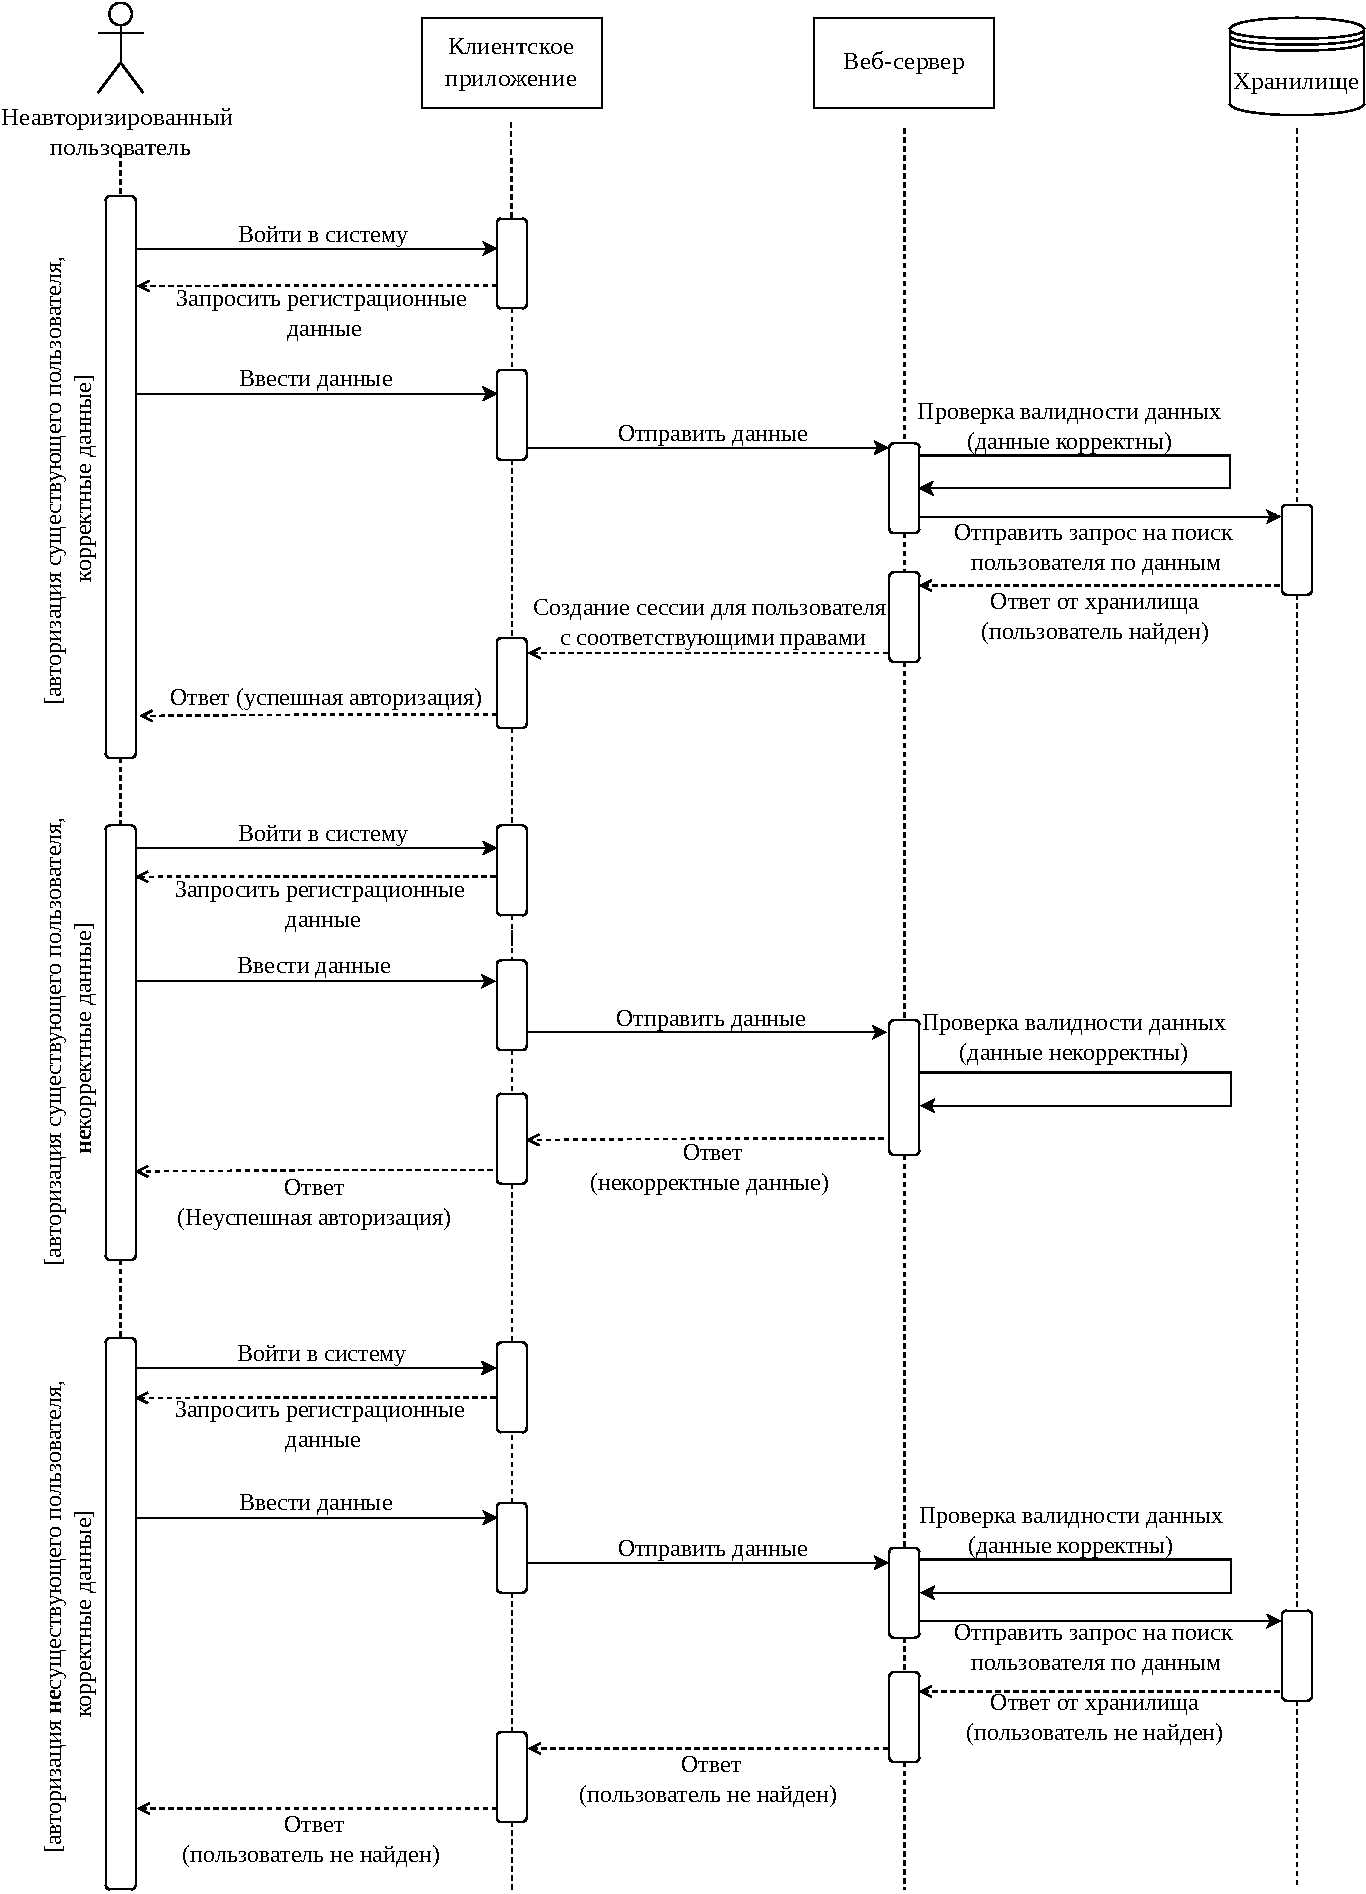
\includegraphics[scale=0.65]{assets/sequence_1.pdf}}
	\caption{Диаграмма последовательности для сценария авторизации пользователя}
\end{figure}

\clearpage

На рисунке 2.7 представлена диаграмма последовательности для сценария создания пациентом заявки на прием.

\begin{figure}[!h]
	\center{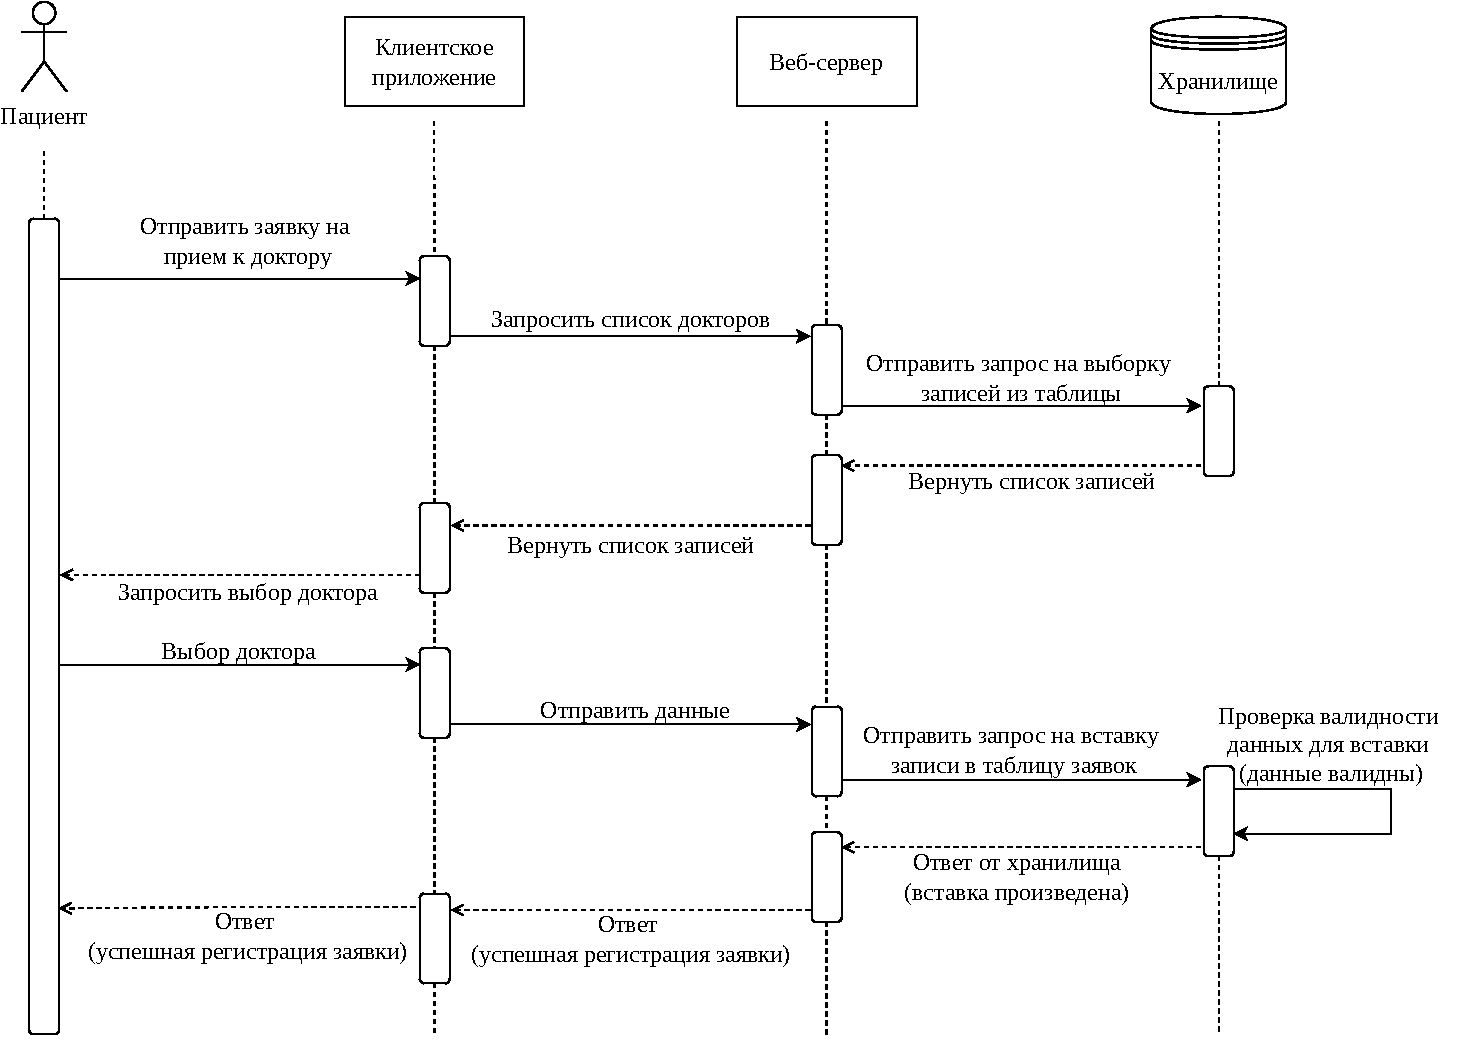
\includegraphics[scale=0.57]{assets/sequence_2.pdf}}
	\caption{Диаграмма последовательности для сценария создания заявки на прием}
\end{figure}

На рисунке 2.8 представлена диаграмма последовательности для сценария просмотра администратором списка докторов в системе.

\begin{figure}[!h]
	\center{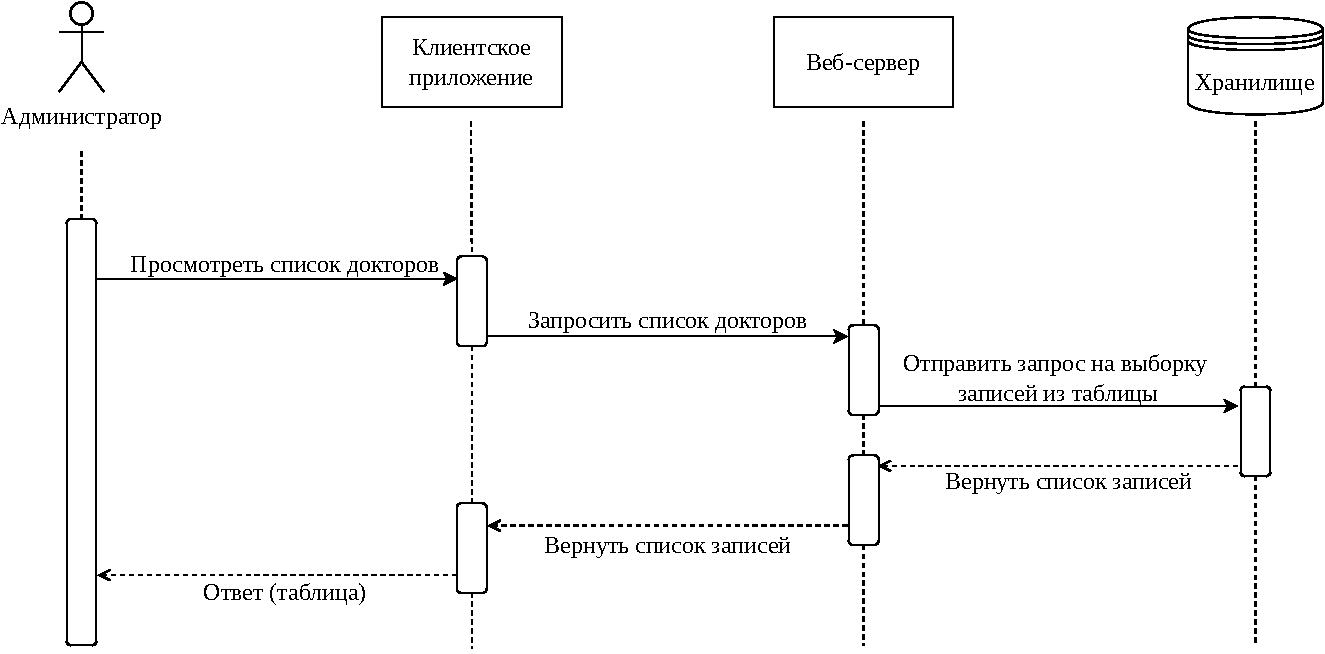
\includegraphics[scale=0.57]{assets/sequence_3.pdf}}
	\caption{Диаграмма последовательности для сценария просмотра списка докторов}
\end{figure}

\clearpage

На рисунке 2.9 представлена диаграмма последовательности для сценария обработки доктором заявки пациента на прием.
\begin{figure}[!h]
	\center{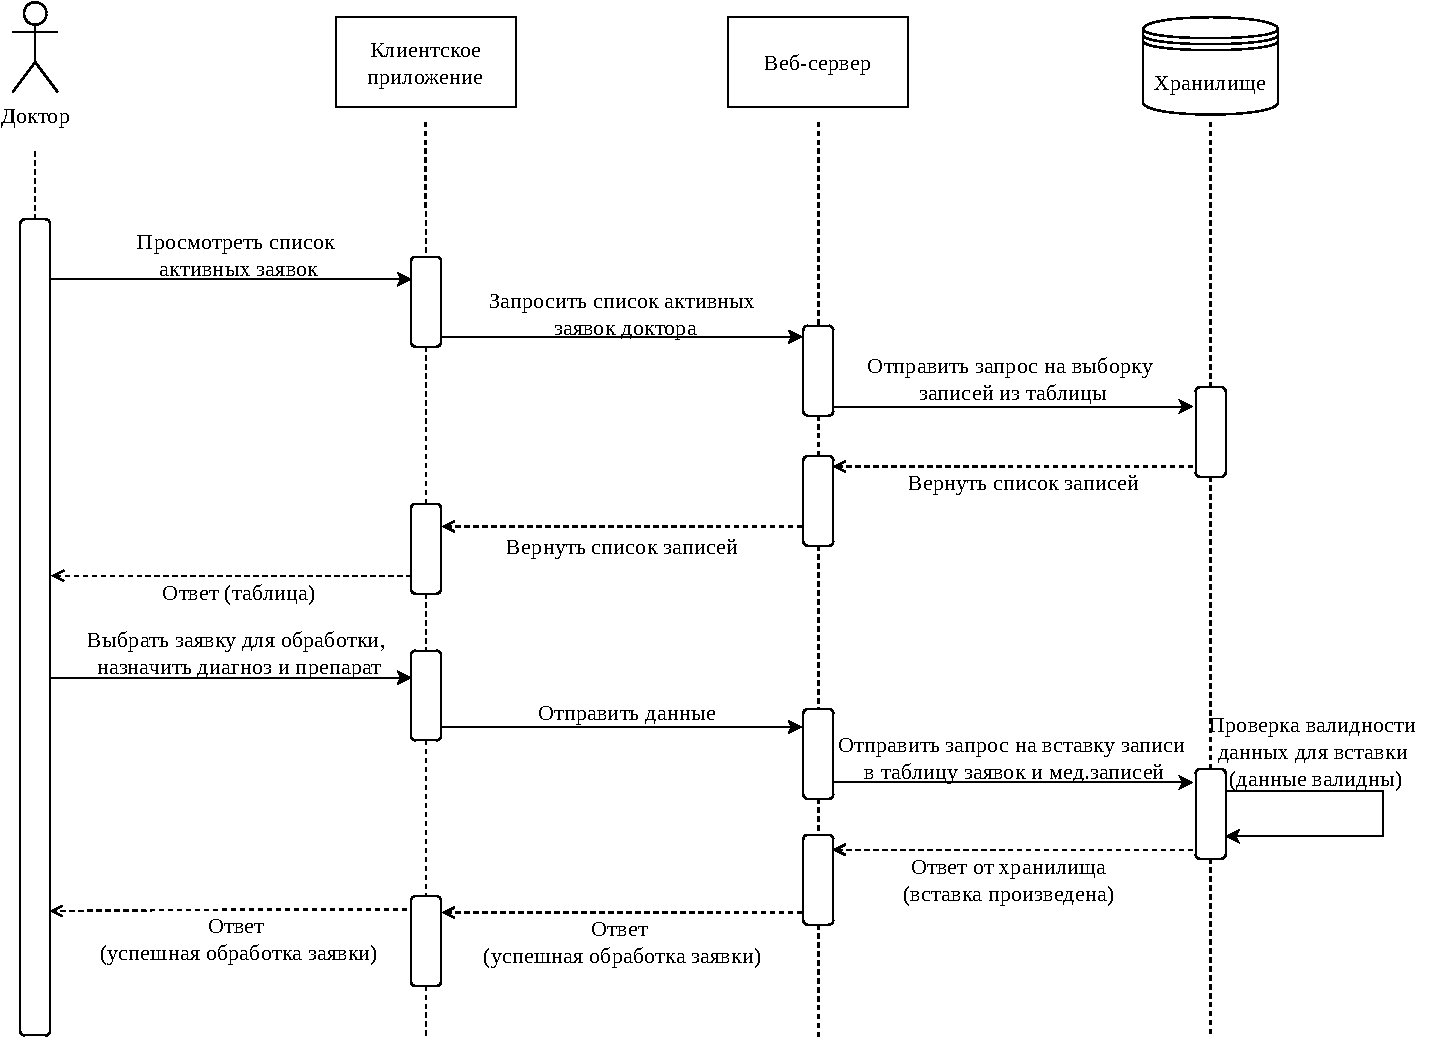
\includegraphics[scale=0.57]{assets/sequence_4.pdf}}
	\caption{Диаграмма последовательности для сценария обработки доктором заявки на прием}
\end{figure}

\clearpage

\section{Описание хранимой функции}

На рисунке 2.10 представлен алгоритм работы хранимой функции, которая подсчитывает статистику заболеваемости (в процентах) для конкретной специализации. Функция возвращает таблицу, содержающую два поля - процент заболеваемости (целое число от 0 до 100) и идентификатор заболевания (целое положительное число).

\begin{figure}[!h]
	\center{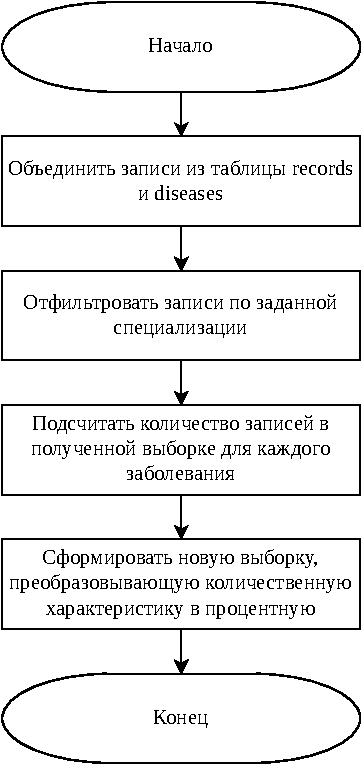
\includegraphics[scale=1]{assets/func.pdf}}
	\caption{Алгоритм работы хранимой функции подсчета статистики заболеваемости}
\end{figure}

\section*{Вывод}

В данном разделе была спроектирована база данных: выделено три типа пользователей, приведены варианты использования системы в соответствии с ролями и представлена диаграмма разрабатываемой системы. В результате разработки должен быть спроектирован сервер, предоставляющий описанный в этом разделе функционал.